\documentclass{article}
\usepackage[T1]{fontenc}
\usepackage[lithuanian]{babel}
\usepackage{graphicx} % Required for inserting images
\usepackage{float} % For accuratelly placing images
\usepackage[a4paper, margin=2cm]{geometry}
\usepackage[hidelinks]{hyperref}
\usepackage{pdflscape}
\usepackage{longtable}
\usepackage{xltabular}
\usepackage{tabularx}
\usepackage{enumitem}

% For striketrghough
\usepackage{soul}

% For colored highlights 
\usepackage{xcolor}

% BEGIN: FOR SVG
% \usepackage[inkscapelatex=false]{svg}
\usepackage{svg}
\usepackage{amsmath}
% END: FOR SVG

\usepackage{everypage}
\usepackage{lscape} % Ensure landscape pages are recognized
\usepackage{lipsum}

\newcommand{\subsubsubsection}[1]{\paragraph{#1}\mbox{}\\}
\setcounter{secnumdepth}{4}
\setcounter{tocdepth}{3}

\title{
    Įmonės „PTN“ procesų gerinimas\\
    \large vertinamas pagal  "AgilityMod" modelį 
    \large versija 2.0 \\
    \large Komanda „PTN“}
\author{
    Greta Virpšaitė \\
    Rugilė Vasaitytė \\
    Domantas Keturakis \\
    Arnas Vaicekauskas \\
    \textbf{Liudas Kasperavičius (Lyderis)} 
}
\date{Spalis 2024}

\begin{document}
% Globals
\newcommand{\WorkProdIdsList}{}
\newcommand{\ProcIdsList}{}

\newcommand{\CheckUniqueWorkProd}[1]{
    \ifinlist{#1}{\WorkProdIdsList} {
    \PackageError{\WorkProdIdsList}{Work product "#1" already exists}{}
    } {
    \ifinlist{#1}{\ProcIdsList} {
        \PackageError{\ProcIdsList}{"#1" exists as a Process}{}
    } {
     \listgadd{\WorkProdIdsList}{#1}
    }
  }
}

\newcommand{\CheckUniqueProc}[1]{
    \ifinlist{#1}{\ProcIdsList} {
    \PackageError{\ProcIdsList}{Work product "#1" already exists}{}
    } {
    \ifinlist{#1}{\WorkProdIdsList} {
        \PackageError{\WorkProdIdsList}{"#1" exists as a Work product}{}
    } {
     \listgadd{\ProcIdsList}{#1}
    }
  }
}

% Work products
\newcommand{\WorkProdList}{}
\newcommand{\defineWorkProduct}[3]{%
  \expandafter\def\csname identifier#1\endcsname{#2}%
  \expandafter\def\csname name#1\endcsname{#3}%
  \CheckUniqueWorkProd{#2}
  \listgadd{\WorkProdList}{#1}
}
\newcommand{\workProdId}[1]{\textit{\csname identifier#1\endcsname}}
\newcommand{\workProdName}[1]{\csname name#1\endcsname}
\newcommand{\workProd}[1]{\workProdId{#1}. \workProdName{#1}}
\newcommand{\prodWork}[1]{\MakeLowercase{\workProdName{#1}} (\workProdId{#1})}

\newcommand{\describeWorkProd}[2]{
    \expandafter\def\csname desc#1\endcsname{#2}
}
\newcommand{\printRow}[1]{
        \workProdId{#1} &
        \workProdName{#1} &
        \csname desc#1\endcsname \\ \hline
}
\newcommand{\workProdDescriptions}{
    \forlistloop{\printRow}{\WorkProdList}
}

% Processes
\newcommand{\defineProcess}[3]{%
  \expandafter\def\csname procId#1\endcsname{#2}%
  \expandafter\def\csname procName#1\endcsname{#3}%
  \CheckUniqueProc{#2}
  \listgadd{\ProcList}{#1}
}
\newcommand{\processId}[1]{\textit{\csname procId#1\endcsname}}
\newcommand{\processName}[1]{\csname procName#1\endcsname}
\newcommand{\process}[1]{\processId{#1}. \processName{#1}}


\maketitle

\newpage
\tableofcontents

\newpage

\section{Pasiruošimas vertinimui}

\subsection{Vertinimo tikslas}

Procesų gerinimas.

\subsection{Vertinimo apimties apibrėžimas}

\subsubsection{Organizacinė apimtis}
Šiame dokumente modeliuojama įmonės "PTN" departamento „Produktų vystymo“ veikla siekiant pagerinti apibrėžtus procesus (žiūrėti \textbf{1.2.3}  dokumento punktą).

\subsubsection{Aukščiausias vertinamas gebėjimo lygis}

Maksimalus vertinimas, kurį gali pasiekti aspektas yra \textbf{trečias}

\subsubsection{Vertinami aspektai}

Vertinami visi "AgilityMod" modelio aspektai: Exploration,  Construction, Transision, Management.

\subsection{Duomenų surinkimas}

Duomenys buvo renkami iš departamento "PTN" \underline{\href{https://github.com/ArnasVaic/software-process/blob/main/PTN.pdf}{procesų aprašymo dokumento}} TODO: NEGALIMA LINK'O Į DOC'Ą turi būti kaip prisegtas failas.

\section{Vertinimas}

\subsection{Aspektų vertinimas}

\href{https://docs.google.com/spreadsheets/d/1unX_xcZLEGHqQOMCuBBXYvVhYjChxpnq/edit?usp=share_link&ouid=113452949406463366361&rtpof=true&sd=true}{vertinimas.xlsx} TODO: NEGALIMA LINK'O Į GOOGLE DOC'Ą turi būti kaip prisegtas failas.

\subsection{Vertinimo rezultatai}

\subsubsection{Lentelė}

\begin{figure}[H]%[htpb!]
    \centering
    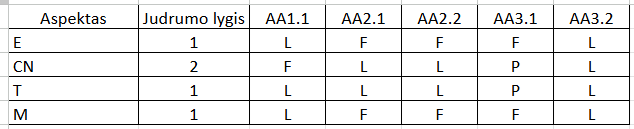
\includegraphics[width=0.85\linewidth]{task-2/images/lentele.png}
\end{figure}

\subsubsection{„Oficialus" judrumo profilis}

\begin{figure}[H]%[htpb!]
    \centering
    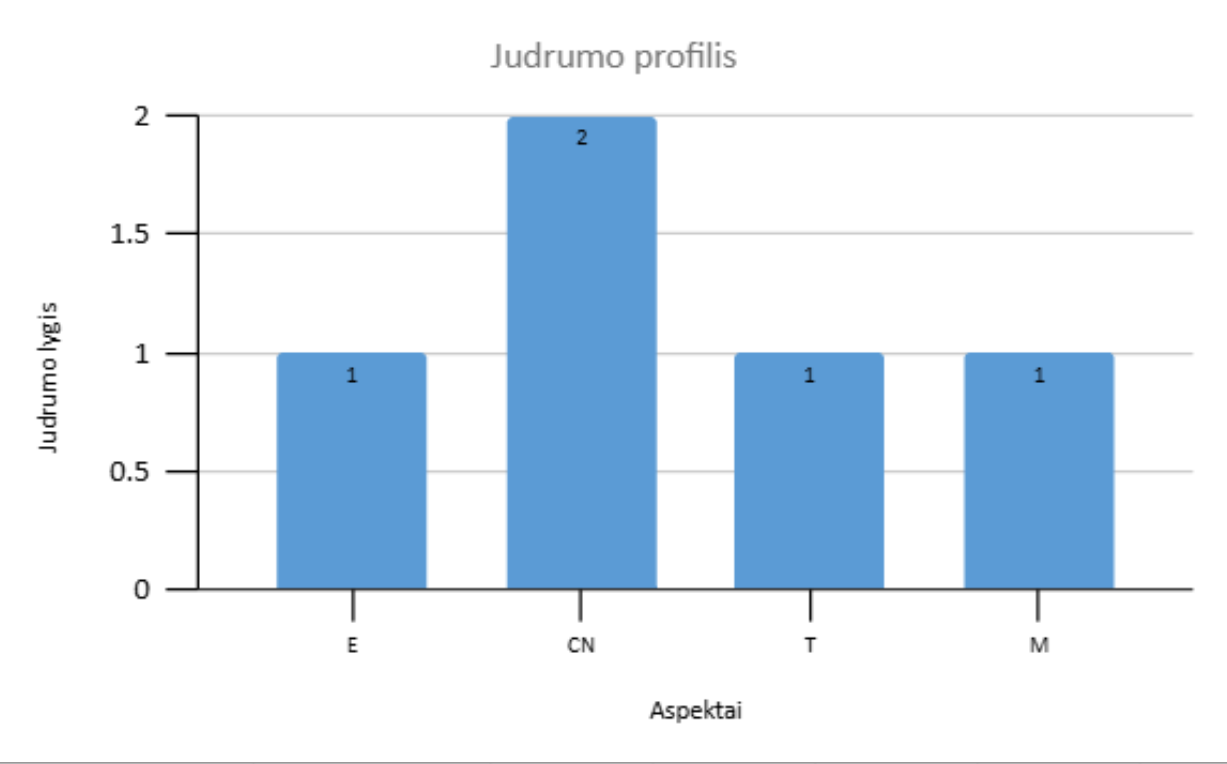
\includegraphics[width=0.85\linewidth]{task-2/images/judrumo-profilis.png}
\end{figure}

\subsubsection{Judrumo profilis gerinimui}

\begin{figure}[h]
    \centering
    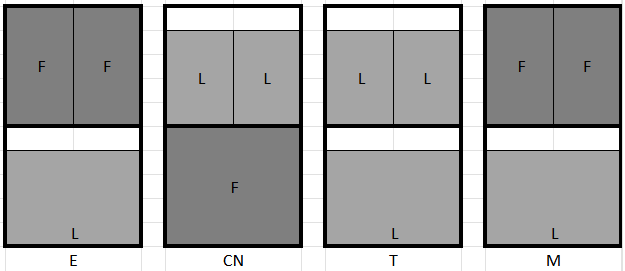
\includegraphics[width=0.75\linewidth]{task-2/images/blokai.png}
    \label{fig:enter-label}
\end{figure}

\section{Gerinimas}

\subsection{Tikslinis judrumo profilis}

\begin{figure}[h]
    \centering
    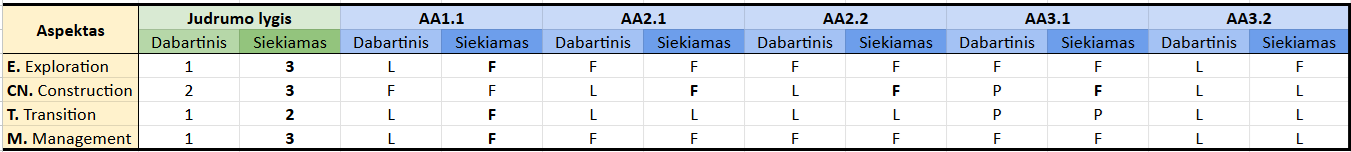
\includegraphics[width=0.75\linewidth]{task-2/images/tikslinis-profilis.png}
    \label{fig:enter-label}
\end{figure}

\newpage
\subsection{Gerinimo veiksmų planas}

\subsubsection{Exploration aspektas}

Šis aspektas pagal esamus procesus yra pasiekęs 1 judrumo lygį. Aspektas gali pasiekti 3 judrumo lygį, jei aspekto atributas
AA 1.1 iš L (77\%) bus pakeltas į F (88\%). Tą pasiekti galima atsižvelgus į šiuo metu procesuose neįgyvendintą E.AP4 aspekto praktiką.

\subsubsubsection{E.AP4 aspekto praktikos įvertinimo N (0\%) gerinimas iki F (100\%) siekiant AA 1.1 F (88\%)}

E.AP4 praktika yra neįgyvendinta N (0\%), ją keliame iki F (100\%) įvykdžius tokius veiklų pakeitimus procesuose:

\subparagraph{Priklausomybių sekimas projekto užduočių sąraše}
\begin{itemize}
    \item \textbf{Vieta:} skyrius 2.3 UR. Užduočių sąrašo rengimas
    \item \textbf{Modifikacija:} pridėti veiklą:
    \begin{quote}
        „Kiekvienai užduočiai (PUS) priskiriamos priklausomybių žymos, nurodant, ar užduotis priklauso nuo kitų užduočių.“
    \end{quote}
\end{itemize}

\subparagraph{Sprinto planavimas (SP)}
\begin{itemize}
    \item \textbf{Vieta:} skyrius 2.4.1 SP. Sprinto planavimas (veikla \#5)
    \item \textbf{Modifikacija:} pridėti prie veiklos:
    \begin{quote}
        „Komanda peržiūri užduotis, kurios priklauso nuo kitų užduočių, užduočių sąraše (SUS) ir užtikrina jų tinkamą prioritetą užduočių sąraše (SUS).“
    \end{quote}
\end{itemize}

\subparagraph{Įgyvendinimo (ĮG) metu keisti priklausomybės statusą}
\begin{itemize}
    \item \textbf{Vieta:} skyrius 2.4.2 ĮG. Įgyvendinimas
    \item \textbf{Modifikacija:} pridėti veiklą:
    \begin{quote}
        „Jeigu rašant programinį kodą, programinės įrangos kūrėjui paaiškėja, kad šios užduoties jis negalės atlikti, nes pirma turi būti atlikta kita užduotis, programinės įrangos kūrėjas sprinto užduočių saraše (\textit{SUS}) pažymi užduotį, nuo kurios priklauso jo atliekama užduotis. Toliau šios užduoties įgyvendinimas nėra tęsiamas iki kol kitos užduoties statusas nepasikeičia į DONE.“
    \end{quote}
\end{itemize}

\subparagraph{Testavimo (TE) metu keisti priklausomybės statusą}
\begin{itemize}
    \item \textbf{Vieta:} skyrius 2.4.3 TE. Testavimas (veikla \#4)
    \item \textbf{Modifikacija:} pridėti prie veiklos:
    \begin{quote}
        „Jei šio proceso metu nebuvo rasta klaidų, užduoties statusas pakeičiamas į DONE. Tuomet automatiškai atnaujinamos visos nuo šios užduoties priklausomos užduotys – jų priklausomybės statusas pakeičiamas į nebeblokuojantį.“
    \end{quote}
\end{itemize}

\subparagraph{Kontrolė (KO)}
\begin{itemize}
    \item \textbf{Vieta:} skyrius 2.4.5 KO. Kontrolė (veikla \#1)
    \item \textbf{Modifikacija:} pridėti prie veiklos:
    \begin{quote}
        „Komanda aptaria iškilusias užduočių priklausomybes (angl. blockers).“
    \end{quote}
\end{itemize}

\newpage
\subsubsection{Construction aspektas}

Aspektas keliamas iš 2 judrumo lygio į 3 judrumo lygį. Tam pasiekti gerinami aspekto atributai:
\begin{enumerate}
\item AA 2.1 iš L (75\%) į F (88\%) 
\item AA 2.2 iš L (75\%) į F (88\%) 
\item AA 3.1 iš P (25\%) į F (96\%) 
\end{enumerate}

\subsubsubsection{
GP 2.1.2 bendrosios praktikos įverčio kėlimas nuo L (75\%) iki F (100\%) siekiant
AA 2.1 aspekto atributo  F (88\%)}

AA 2.1 atributas pagerinamas nuo L (75\%) iki F (88\%), pakėlus GP 2.1.2 bendrosios praktikos įvertį nuo 75\% iki 100\%. Tam procesuose atlikti šie pakeitimai: \\


\subparagraph{Kasdieniai Stand-Up susitikimai}
\begin{itemize}
    \item \textbf{Vieta:} skyrius 2.4.2 ĮG. Įgyvendinimas
    \item \textbf{Modifikacija:} pridėti naują veiklą
    \begin{quote}
    „Kiekvieną dieną komanda rengia trumpą Stand-Up susitikimą, kad aptartų progresą, nustatytų kliūtis ir sinchronizuotų veiklas tarp komandos narių. Šis susitikimas įprastai trunka ne ilgiau kaip 15 minučių ir susideda iš trijų pagrindinių punktų: kas buvo padaryta vakar, kas bus daroma šiandien, ir su kokiomis kliūtimis susiduriama.“
    \end{quote}
\end{itemize}


\subparagraph{Komunikacijos įrankių naudojimas}
\begin{itemize}
    \item \textbf{Vieta:} skyrius 2.4.1 SP. Sprinto planavimas (veikla \#5)
    \item \textbf{Modifikacija:} pakeisti veiklą 
    \begin{quote}

     „Sprinto užduočių sąrašas (SUS) realizuojamas visai komandai ir SŠ matomomis „Kanban“ lentomis.“
    \end{quote}
\end{itemize}

% \subparagraph{Dokumentuoti komunikaciją Kontrolės (KO) procesese}
% \begin{itemize}
%     \item \textbf{Vieta:} skyrius 2.4.5 KO. Kontrolė
%     \item \textbf{Modifikacija:} pridėti veiklą
%     \begin{quote}
%     % įvertina komunikacijos     kasdienius Stand-Up susitikimus ir tokių
% % kaip „Kanban“ lentos, „Slack“ ir kt. naudojimo, efektyvumą. Komanda aptaria iškilusius priklausomybiu ̨ blokatorius. Visi komandos nariai surašo savo atsiliepimus. \\
%         „Sprinto retrospektyvos metu komandos nariai įvertina komunikacijos praktikų, įskaitant kasdienius Stand-Up susitikimus ir tokių įrankių kaip Kanban lentos ir Slack naudojimo, efektyvumą. Šis grįžtamasis ryšys dokumentuojamas Sprinto Peržiūros Ataskaitoje (SPA), siekiant nuolat gerinti komunikacijos praktikas.“
%     \end{quote}
% \end{itemize}

\subparagraph{Komunikacijos priemonės pristatant SŠ}
\begin{itemize}
    \item \textbf{Vieta:} skyrius 2.4.4 PAS. Pristatymas ir grįžtamojo ryšio surinkimas
    \item \textbf{Modifikacija:} pridėti prie veiklos
    \begin{quote}
        „Tai gali vykti nuotoliniu būdu arba gyvo susitikimo metu, per kurį naudojami įvairūs informacijos radiatoriai, pvz: skaidrės, projektoriai, rašomosios lentos ir t. t.“
    \end{quote}
\end{itemize}

\subsubsubsection{GP 2.2.2 gerinimas nuo L (75\%) iki F (100\%), siekiant AA 2.2 F (88\%) įverčio.}

Procesuose yra kuriama techninė dokumentacija ir produkto naudojimo instrukcija. Produkto naudojimo instrukcijos rašymas yra vieną kartą projekte vykstantis procesas, tuo tarpu techninė dokumentacija rašoma įgyvendinimo metu. Norint taikyti „minimalią ceremoniją“, prieš rašant dokumentaciją reikia įvertinti, ar įgyvendintai užduočiai dokumentacijos rašymas yra būtinas.

\subparagraph{Kriterijai techninei dokumentacijai}
\begin{itemize}
    \item \textbf{Vieta:} skyrius 2.4.2  ĮG. Įgyvendinimas
    \item \textbf{Modifikacija:} nauja veikla -- techninės dokumentacijos poreikio įvertinimas.
    \begin{quote}
    „Vykdomas techninės dokumentacijos poreikio įvertinimas. Vertinama pagal šiuos kriterijus: \textbf{konfigūracija} -- ar užduoties rezultatas konfigūruojamas produkto konfigūraciniuose failuose, \textbf{išoriškumas} -- ar užduoties rezultatas pasiekiamas išoriniams vartotojams (pvz. API), \textbf{kritiškumas} -- užduoties rezultato poveikis bendram produkto funkcionalumui.“
    \end{quote}
\end{itemize}
\vspace{15pt}
\begin{itemize}
    \item \textbf{Vieta:} skyrius 2.4.2  ĮG. Įgyvendinimas (veikla \#8)
    \item \textbf{Modifikacija:} Pridėti prie veiklos
    \begin{quote}
    „Techninė dokumentacija užduočiai rašoma tik jei jos poreikio vertinimas teigiamas.“
    \end{quote}
\end{itemize}

\subsubsubsection{GP 3.1.1 bendrosios praktikos gerinimas nuo P (25\%) iki F (100\%) seikiant AA 3.1 aspekto  F (96\%)}

Norint pasiekti F įvertinimą aspekto atributui AA 3.1, GP 3.1.1 atlikti šie pakeitimai, praktiką pakeliant nuo P (25\%) iki F (100\%):

\subparagraph{Integruoti TDD}
\begin{itemize}
    \item \textbf{Vieta:} skyrius 2.4.2 ĮG. Įgyvendinimas (veikla \#4)
    \item \textbf{Modifikacija:} Perkelti modulių testų rašymo žingsnį prieš kodo rašymo, ir pridėti reikalavimą programinės įrangos kūrėjų naudoti TDD metodiką.
    \begin{quote}  „Programinės įrangos kūrėjai pritaiko testų kūrimo metodą (TDD), prieš pradedant kurti funkcionalumą. TDD užtikrina, kad kiekviena funkcija būtų padengta modulių testais, siekiant išvengti klaidų ir garantuoti kodo kokybę. Laikoma, kad yra atnaujinamas programinis kodas (PK).“
    \end{quote}
\end{itemize}

\subparagraph{Programavimas poromis veikla}
\begin{itemize}
    \item \textbf{Vieta:} skyrius 2.4.2 ĮG. Įgyvendinimas
    \item \textbf{Modifikacija:} Pridėti naują veiklą
    \begin{quote} „Sudėtingas arba itin svarbias užduotis programinės įrangos kūrėjai dalinai atlieka porose. Darbo porose tikslas - dalintis žiniomis ir efektyvesnė kodo peržiūra.“
    \end{quote}
\end{itemize}

\newpage
\subsubsection{Transition aspektas}

Šis aspektas pagal esamus procesus yra pasiekęs 1 judrumo lygį. Aspektas gali pasiekti 2 judrumo lygį, jei aspekto 
atributas AA 1.1 iš L (77\%) bus pakeltas į F (88\%).


\subsubsubsection{T.AP1 aspekto praktikos gerinimas nuo P (40\%) iki L (80\%)}

Išskirti praktikos trūkumai yra tie, jog artefaktai ir trečių šalių bibliotekos nėra saugomos tam skirtose saugyklose, be to, testavimo aplinkos nėra išskirtos ir nėra valdomos.

\subparagraph{Aplinkos rengimas}
\begin{itemize}
    \item \textbf{Vieta:} 2.4 AR. Aplinkos rengimas 
    \item \textbf{Modifikacija:} Pridėtas naujas procesas aplinkos kūrimui aprašyti. 

    \begin{quote}
    \begin{longtable}{p{0.1\textwidth}|p{0.9\textwidth}}
        AP & Aplinkos paruošimas \\ \hline
        Tikslas & Paruošti kodo repozitoriją. Automatizuoti kodo testavimo bei diegimo procesą. \\ \hline
        Panaudoti darbo produktai & \begin{itemize}
            \item ALSA. Aukšto lygio sistemos architektūra
        \end{itemize} \\ \hline
        Sukurti darbo produktai &
        \begin{itemize}
            \item PK. Programinis kodas
            \item AP. Aplinka
        \end{itemize}
        \\ \hline
        Veiklos & \begin{enumerate}
            \item Architektas atsižvelgdamas į aukšto lygio architektūrą (ALSA) sukuria kodo repozitoriją, kurioje bus saugomas programinis kodas (PK), trečių šalių bibliotekų ir diegimo konfigūracija. Pagal pasirinkto karkaso (pavyzdžiui: .NET, Spring Boot) šabloną  sukuria pirminį projekto programinį kodą.
    
            \item Architektas parengia saugyklą trečių šalių bibliotekoms saugoti.
    
            \item Architektas sukuria ir parengia testavimo aplinką (AP).
    
            \item Architektas ruošia trečiųjų šalių bibliotekų saugyklas ir konfigūruoja CI/CD - užtikrina, kad sukūrus naują programinio kodo versiją būtų paleidžiami automatiniai testai, jiems suveikus be klaidų, nauja produkto versija automatiškai sudiegiama į testavimo aplinką (AP).
       \end{enumerate}
    \end{longtable}
    \end{quote}
\end{itemize}

\vspace{10pt}
\begin{itemize}
    \item \textbf{Vieta:} skyrius 3 Darbo produktų sąrašas
    \item \textbf{Modifikacija:} Pridėti naują darbo produktą
    \begin{itemize}
        \item Id: AP
        \item Pavadinimas: Aplinka
        \item Aprašymas: „Infrastruktūra, kurioje vykdomas testavimas ir diegiamas programinis kodas, laikoma konfigūracija.“
    \end{itemize}
\end{itemize}

\subsubsubsection{T.AP2 aspekto praktikos kėlimas nuo L (60\%) iki F (100\%)}

Kodo integravimas turėtų vykti pusiau automatiškai (kodo konfliktų sprendimas negali būti visiškai automatizuotas). Artefaktų kūrimas turėtų būti automatizuotas (padengta nauju procesu).

\subparagraph{Automatinis integravimas}
\begin{itemize}
    \item \textbf{Vieta:} skyrius 2.4.2 ĮG. Įgyvendinimas (veikla \#5)
    \item \textbf{Modifikacija:} Pakeisti veiklą
    \begin{quote}
    „Programinės įrangos kūrėjas, atsakingas už užduotį, keičia užduoties statusą į \mbox{IN~REVIEW}. Auotomatiškai prasideda kodo integracija ir diegimas į testavimo aplinką (CI/CD). Jei integracija ar diegimas nesėkmingi (yra kodo konfliktų su pagrindine kodo šaka arba ne visi testai teigiami), užduoties statusas automatiškai grąžinamas į \mbox{IN~PROGRESS}, progrminės įrangos kūrėjas, atsakingas už užduotį ištaiso klaidas ir veikla kartojama tol, kol CI/CD įvyksta sėkmingai.“
        % „Jeigu yra konfliktų su pagrindine programinio kodo atšaka -- juos pataiso. Papildomai, programinės įrangos kūrėjas įsitikinima, kad testų rezultatai (automatiškai sugeneruojami CI/CD infrastruktūros) yra teigiami. Tik tada, programinės įrangos kūrėjas, atsakingas už užduotį, keičia užduoties statuso atributą į \mbox{IN~REVIEW}.
    \end{quote}
   %  \begin{quote}
   % Kodo integracija vykdoma naudojant XXXX, kurios automatiškai sukuria artefaktus ir paleidžia regresinius testus po kiekvieno kodo pakeitimo. Kodo konfliktų sprendimas, jei reikia, vykdomas rankiniu būdu, siekiant užtikrinti kodo vientisumą ir suderinamumą.
   %  \end{quote}
\end{itemize}
\vspace{10pt}

\begin{itemize}
    \item \textbf{Vieta:} skyrius 2.4.4 „Pristatymas ir grįžtamojo ryšio surinkimas“ (veikla \#1)
    \item \textbf{Modifikacija:} Pašalinti veiklą
\end{itemize}
\vspace{20pt}
\begin{itemize}
    \item \textbf{Vieta:} skyrius 2.4.4 „Pristatymas ir grįžtamojo ryšio surinkimas“ (veikla \#2)
    \item \textbf{Modifikacija:} Pakeisti veiklą
    \begin{quote}
        „Programinės įrangos kūrėjas pristato naujasią produkto versiją (PROD), įdiegtą testavimo aplinkoje (AP), suinteresuotoms šalims.“
    \end{quote}
\end{itemize}

\subsubsubsection{T.AP3 bendrosios praktikos gerinimas nuo P (50\%) iki F (100\%)}

Diegimas į visas aplinkas vyksta rankiniu būdu, o ne automatiniu.

Padengtas nauju procesu aprašytu 3.2.3.1.

\subsubsubsection{T.AP4 bendrosios praktikos gerinimas nuo F (90\%) iki F (100\%)} 

\subparagraph{Regresiniaitestai turi būti automatizuoti.}
\begin{itemize}
    \item \textbf{Vieta:} skyrius 2.4.3 Testavimas
    \item \textbf{Modifikacija:} Pridėti naują veiklą
    \begin{quote}
    „Automatizuotus regresinius testus kuria ir rašo testuotojas, kuris yra atsakingas už testų kūrimo ir priežiūros procesą. Šie testai užtikrina, kad kodo pakeitimai nesukelia klaidų ir nepažeidžia esamo funkcionalumo. Laikoma, kad atnaujintas programinis kodas (PK).“
    \end{quote}
\end{itemize}

% \subsubsubsection{T.API5: Padaryti progresą matomu (angl. „Make the Progress Visible“)}

% Užduoties dokumente neatsispindi aplinka, kurioje šiuo metu yra su užduotimi susijęs kodas

% Nėra vieno dokumento (pvz. Jira ar Github platformoje), kuris atspindi dabartinę kiekvienos aplinkos būklę (t. y. koks kodas yra sudiegtas) 
\newpage

\subsubsection{Management aspektas}

Šis aspektas pagal esamus procesus yra pasiekęs 1 judrumo lygi. Aspektas gali pasiekti 3 judrumo lygį, jei
aspekto atributas AA 1.1 iš L(82\%) bus pakeltas į F(87\%).

Pasiekti 3 judrumo lygį galime pakelti M.AP1 aspekto praktikos įvertinimą L (51\%) ir M.AP8 aspekto praktikos įvertinimą L(80\%) iki F(100\%).

\subsubsubsection{M.AP1 aspekto praktikos gerinimas nuo L (51\%) iki F (100\%)}
\vspace{-15pt} %XDDDD
\subparagraph{Pagrįstumo analizė}
\begin{itemize}
    \item \textbf{Vieta:} skyrius 2.1 KĮ. Kliento įtraukimas (veikla \#2).
    \item \textbf{Modifikacija:} pataisyti veiklą ir ją išskirti į dvi:
    \begin{quote}
        „Projektų vadovas, architektas ir analitikas paruošia pradinė projekto viziją tam, kad būtų patvirtintas projekto įgyvendinamumas ir suderinta bendra projekto kryptis su SŠ. Jie taip pat atlieka pagrįstumo analizę, siekdami įvertinti, ar kliento poreikiai (KP) yra įgyvendinami." 
    \end{quote}
    
    \begin{quote}
        „Projektų vadovas, architektas ir analitikas  atsižvelgdami į projekto viziją, pagrįstumo analizę, departamento patirtį su kitais projektais (PAT) bei projekto apimtimi (PA) nustato laiko, kainos ir žmogiškųjų išteklių sąmatą (IS). Laikas, kaina (nustatyti iš IS), projekto apimtis (PA), produkto perdavimo sąlygos ir adaptacinio laikotarpio terminas tuomet yra teisiškai įforminami sutartyje (KS)."
    \end{quote}
\end{itemize}

\subsubsubsection{M.AP8 aspekto praktikos gerinimas nuo L (80\%) iki F (100\%)}

\subparagraph{Rizikų įvertinimas}
\begin{itemize}
    \item \textbf{Vieta:} skyrius 2.1 KĮ. Klientų įtraukimas
    \item \textbf{Modifikacija:} pridėti veiklą
    \begin{quote}
        „Analitikas identifikuoja ir įvertina projekto rizikas, pagal jas sukuria rizikų valdymo planą (RVP).“
    \end{quote}
\end{itemize}

\vspace{10pt}
\begin{itemize}
    \item \textbf{Vieta:} skyrius 3 Darbo produktų sąrašas
    \item \textbf{Modifikacija:} Pridėti naują darbo produktą
    \begin{itemize}
        \item Id: RVP
        \item Pavadinimas: Rizikų valdymo planas
        \item Aprašymas: Rizikų valdymo planas yra dokumentas, kuriame identifikuojamos, vertinamos ir aprašomos galimos projekto rizikos. Planas apima rizikų identifikavimo metodus, rizikų vertinimo kriterijus, rizikų prioritetų nustatymą bei rizikų mažinimo ir valdymo strategijas. Be to, jame nurodomos atsakomybės už rizikų valdymą, rizikų stebėjimo procedūros ir komunikacijos planas su suinteresuotomis šalimis.
    \end{itemize}
\end{itemize}

\subparagraph{Rizikų sekimas}
\begin{itemize}
    \item \textbf{Vieta:} sekcija 2.4.5 KO. Kontrolė
    \item \textbf{Modifikacija:} pridėti veiklą:
    \begin{quote}
        „Projekto vadovas vykdo stebėseną ir esant reikalui švelnina rizikas arba vykdo žalos kontrolę pagal rizikų valdymo planą (RVP).“
    \end{quote}
\end{itemize}

\end{document}
